\documentclass{seminar}
\usepackage{epic,/homes/tiwari/Talks/Special/relative,latexsym,url}
\usepackage{/homes/tiwari/Talks/Special/gastex}
\usepackage{wrapfig}

\usepackage{fancybox}
\usepackage{semlayer}
\usepackage{epsfig}
\usepackage{amssymb}
\usepackage{semcolor}

\def\printlandscape{\special{landscape}}    % Works with dvips.
\renewcommand{\printlandscape}{\special{landscape}}
\special{! /landplus90 true store}

\input{/homes/tiwari/Talks/Special/slideprel}
\slideframe{oval}
\usepackage{times} 		%% for PDF purposes

\newcommand\ignore[1]{{{}}}

% \ifpdf\else
%%%%%%%%
% to fix problems making landscape seminar pdfs
% Letter...
%\pdfpagewidth=11truein
%\pdfpageheight=8.5truein
% A4
\pdfpagewidth=297truemm % your milage may vary....
\pdfpageheight=210truemm
\pdfhorigin=1truein     % default value(?), but doesn't work without
\pdfvorigin=1truein     % default value(?), but doesn't work without
%\fi
% -------------------------------------------------------

%---------------------------------------------------------------------
\begin{document}
%---------------------------------------------------------------------
\begin{slide}
\heading{HybridSAL: Tool for Analyzing Hybrid Systems}
\heading{Using Relational Abstraction}

{\cem{Background}}: 
 Few {\crm{automated tools}} for verifying systems with 
 {\crm{mixed discrete and continuous dynamics}}, and 
 {\cem{none}} are {\cem{compositional}}

\bigskip
{\cem{Accomplishment}}:
 We have developed {\cem{two new}} techniques for analyzing
 {\cem{open components}} based on
 \begin{itemize}
 \item 
  {\cem{certificate-based techniques}} for generating {\cem{assume-guarantee pairs}}
 \item
  {\cem{relational abstractions}}
 \end{itemize}

\end{slide}
% -------------------------------------------------------
\begin{slide}
\heading{HybridSAL Supports Relational Abstraction}

{\crm{Progress}}:
 {\cem{The HybridSAL tool can construct relational abstractions}}

\bigskip

\begin{tabular}{p{1in}@{$\quad\Leftarrow\quad$}p{1in}@{$\quad\Rightarrow\quad$}p{0.8in}}
\hline
\multicolumn{1}{c}{\crm{HybridSAL}}
&
\multicolumn{1}{c}{\crm{HybridSAL}}
&
\multicolumn{1}{c}{\crm{HSAL}}
\\
\multicolumn{1}{c}{\crm{Abstractor}}
&
\multicolumn{1}{c}{}
&
\multicolumn{1}{c}{\crm{RelAbstractor}}
\\
\hline\hline
Constructs {\cem{qualitative abstractions}} of 
HybridSAL models
&
{\cem{Formal language}} for describing
systems with {\cem{hybrid dynamics}}
&
Constructs {\cem{relational abstractions}} of 
HybridSAL models
\\
\hline
\multicolumn{1}{c}{Finite state$\hfill$ Old}
&
\multicolumn{1}{c}{$\hfill$ New}
&
\multicolumn{1}{c}{Infinite state}
\\
\hline
\end{tabular}

\end{slide}
% -------------------------------------------------------
\begin{slide}
\heading{HSAL Relational Abstractor}

The {\cem{use case}}:

\begin{enumerate}
\item
 User creates a {\cem{HybridSAL model}} of the system/component of interest
 \begin{itemize}
 \item Using a text editor
 \item From Vanderbilt's CyPhy environment
 \end{itemize}
 Model resides in {\cem{filename.hsal}}

\item
 User adds {\cem{properties}} of interest  to the model
 \\
 Properties also go inside {\cem{filename.hsal}}

\item
 {\cem{HSal RelAbstractor}} automatically constructs {\crm{filename.sal}}

\item
 Sal model checkers can be used to verify {\crm{filename.sal}}
 \\
 {\texttt{sal-inf-bmc -i -d 5 filename property}}
\end{enumerate}

\medskip
These steps can be seen in the {\crm{demo}} 

\end{slide}
% -------------------------------------------------------
\begin{slide}
\heading{HSAL Relational Abstractor}

Is developed {\cem{compositionally}}

Independently usable {\cem{components of HSAL Relational Abstractor}}:
\begin{itemize}
\item
 {\cem{hsal2hxml}}:  A parser for HybridSAL, creates HSAL model in XML
\item
 {\cem{hxml2hsal}}:  Pretty printer for HSAL XML
\item
 {\cem{hsal2hasal}}:  HSal relational abstractor, from .hsal, or .hxml to .hasal
\\
 The original model and its abstraction are {\cem{both}} stored in .hasal file
\\
 hsal2hxml can parse .hasal file
\\
 hxml2hsal can also pretty print .haxml file
\item
 {\cem{hasal2sal}}:  Extract the abstract SAL model from .hasal file
\end{itemize}

\medskip
{\cem{Key Idea}}: {\crm{Enriched components}}, .hasal file stores
 {\cem{components, properties, and abstractions}}

\end{slide}
% -------------------------------------------------------
\begin{slide}
\heading{Relational Abstraction: Concept}

Consider a dynamical system $(X, \rightarrow)$
where
\begin{tabular}{l@{:}l}
$X$ & variables defining {\cem{state space}} of the system
\\
$\rightarrow$ & binary relation over state space defining {\cem{system dynamics}}
\end{tabular}

\medskip
We do not care if 
\begin{itemize}
\item
the system is {\cem{discrete-}} or {\cem{continuous-}} or {\cem{hybrid-time}}, or 
\item
the system
has a {\cem{discrete}}, {\cem{continuous}}, or {\cem{hybrid state space}}
\end{itemize}

\medskip
For discrete-time systems, $\rightarrow$ is the one-step transition relation
\\
For continuous-time systems, $\rightarrow = \cup_{t\geq 0} \stackrel{t}{\rightarrow}$ 
where
$\stackrel{t}{\rightarrow}$ 
is the transition relation corresponding to an elapse of $t$ time units

\end{slide}
% -------------------------------------------------------
\begin{slide}
\heading{Relational Abstraction: Concept}

Relational abstraction of
a dynamical system 
$(X, {\cem{\rightarrow}})$
is another dynamical system
$(X, {\crm{\rightarrow}})$
such that
$$
\mbox{TransitiveClosure}({\cem{\rightarrow}})  \;\subseteq\; {\crm{\rightarrow}}
$$

\medskip
{\cem{Relational Abstraction:}}
An over-approximation of the transitive closure of the transition relation

\bigskip
{\cem{Benefit:}}
\\
Eliminates need for iterative fixpoint computation 
\\
Useful for proving safety properties, and establishing
conservative safety bounds

\end{slide}
% -------------------------------------------------------
\begin{slide}
\heading{Relational Abstraction: Example}

For the continuous-time continuous-space dynamical system:
\begin{eqnarray*}
 \frac{dx}{dt} & = & -x + y
\\
 \frac{dy}{dt} & = & -x - y
\end{eqnarray*}

we have the following continuous-space discrete-time relational abstraction:
\begin{eqnarray*}
(x,y) \;{\crm{\rightarrow}}\; (x',y')  & := &
   \mathtt{max}(|x|,|y|) \geq 
   \mathtt{max}(|x'|,|y'|)
\end{eqnarray*}

If initially $x \in [0,3], y \in [-2,2]$, then in {\cem{any}} future time,
$x,y$ will remain in the range $[-3,3]$


\end{slide}
% -------------------------------------------------------
\begin{slide}
\heading{Relational Abstraction: Challenge}

Is it possible to {\cem{compute}} relational abstractions?

\bigskip

We do {\cem{not}} want to abstract discrete-time transition relations,
because model checkers (and static analyzers) can handle them (compute fixpoint)

\bigskip
Is it possible to {\cem{compute}} relational abstractions of
continuous-time dynamics?

\end{slide}
% -------------------------------------------------------
\begin{slide}
\heading{Computing Relational Abstractions}

We have an {\cem{algorithm}} for computing relational abstractions
of {\cem{linear}} systems

\bigskip

\begin{tabular}{|l|l|}
\hline
Dynamics & Relational Abstraction
\\
\hline \hline
$\dot{x} = 1, \dot{y} = 1$
&
$x'-x = y'-y$
\\
\hline
$\dot{x} = 2, \dot{y} = 3$
&
$(x'-x)/2 = (y'-y)/3$
\\
\hline
$\dot{\vec{x}} = A\vec{x}$
&
$(0 \leq p' \leq p) \vee (0 \geq p' \geq p)$, where
\\
&
$p = \vec{c}^T\vec{x}$, $\vec{c}$ eigenvector
of $A^T$ corr. to negative eigenvalue
\\
\hline
$\dot{\vec{x}} = A\vec{x} + \vec{b}$
& 
$\ldots$
\\
\hline
\end{tabular}

\medskip
Why are such simple dynamics important?
\\
{\cem{Timed}} automata, 
{\crm{Multirate}} automata, {\cem{linear hybrid}} systems

\end{slide}
% -------------------------------------------------------
\begin{slide}
\heading{Computing Relational Abstractions}

For linear systems, we can use plenty of linear algebra
to {\cem{automatically}} generate relational abstractions

\medskip
More generally, we can use the {\cem{certificate-based}} approach to generate
relational abstractions using {\cem{constraint solving}}

\medskip
By fixing a {\cem{form}} for the relational abstraction,
we can find the abstraction by solving an {\cem{$\exists\forall$}} formula

\medskip
The algorithm for creating relational abstractions of linear systems
can be viewed as
a special case of this generic method, where the
$\exists\forall$ problems are being solved using linear algebra tricks.

\end{slide}
% -------------------------------------------------------
\begin{slide}
\heading{Relational Abstraction: Summary}

\begin{tabular}{c|c}
\begin{minipage}{1.8in}
\begin{description}
\item[Benefit:] Enables analyzability of complex systems
\\
\hspace*{-2em}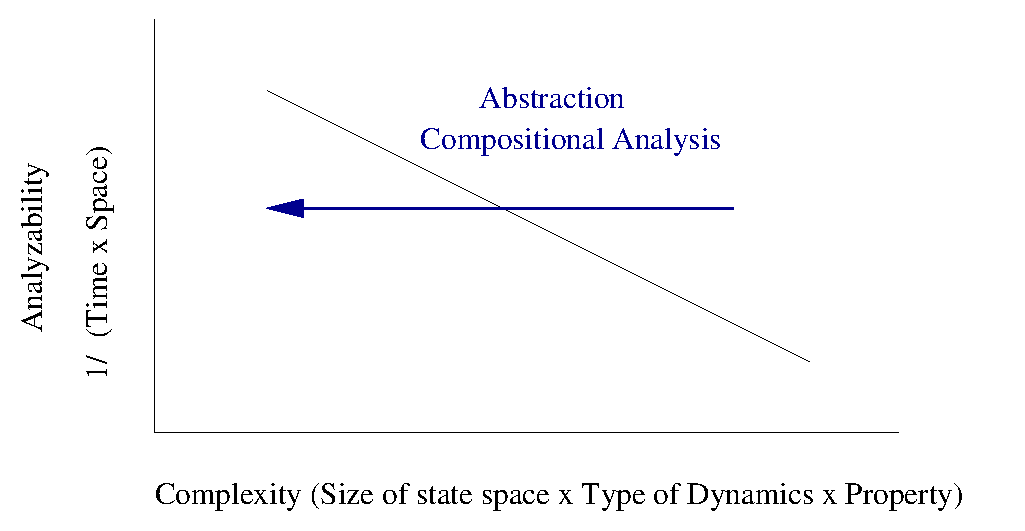
\includegraphics[angle=0,scale=0.3]{reduceComplexity}

\item[Feature:] Compositional analysis: Abstracts open components
 with hybrid dynamics

\item[Feature:] Compatible with other abstraction and model checking
 techniques
\end{description}
\end{minipage}
&
\begin{minipage}{2.1in}
\begin{description}
\item[Novelty:] Abstracts the transition relation, not the state space
\\
\hspace*{-1em}
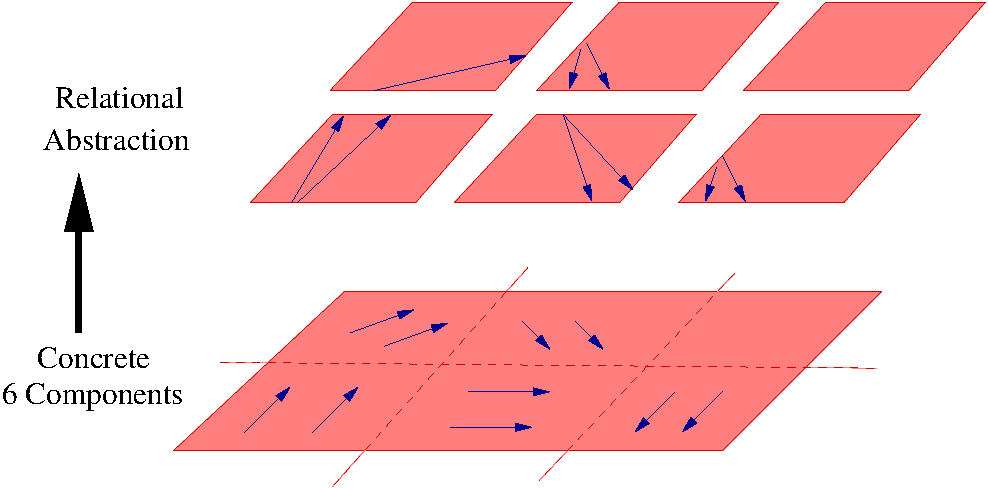
\includegraphics[angle=0,scale=0.35]{relabsnew}

\item[Scope:] Applies to all dynamical systems. Effective relational
 abstractions can be computed for several classes.
\end{description}
\end{minipage}
\end{tabular}

\end{slide}
% -------------------------------------------------------
\begin{slide}
\subheading{Relational Abstraction: Examples}

\begin{tabular}{c|c|c}
\begin{minipage}{1.3in}
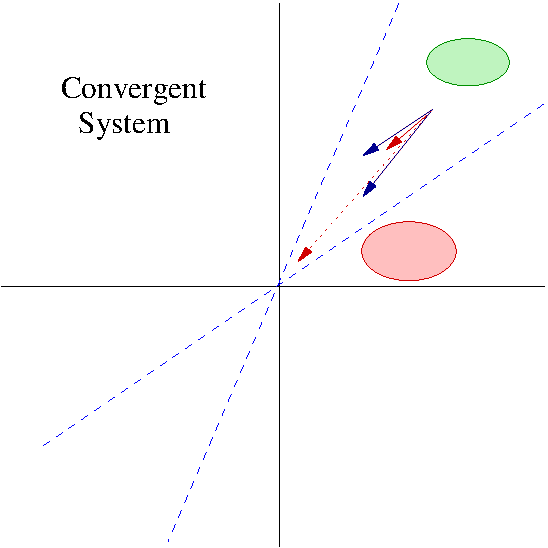
\includegraphics[angle=0,scale=0.3]{conv}
\\
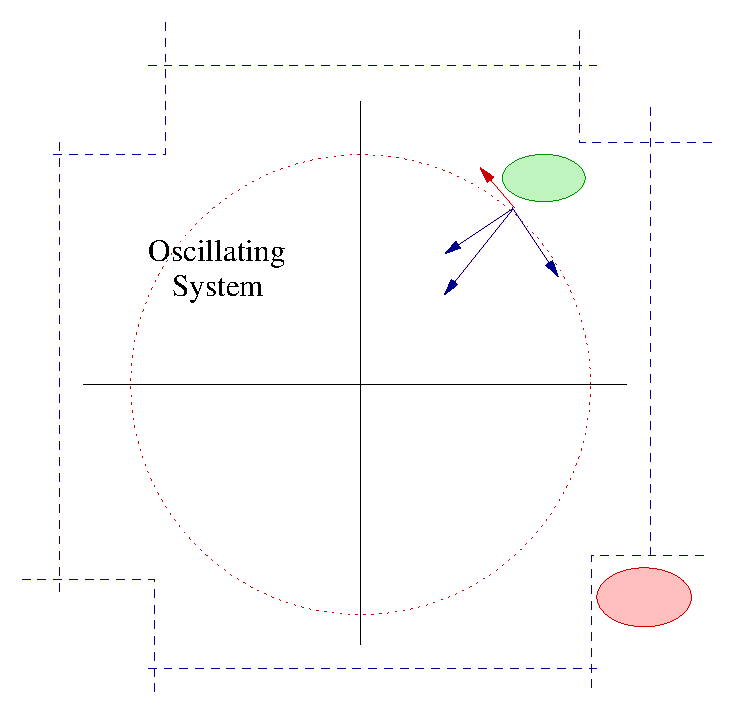
\includegraphics[angle=0,scale=0.3]{osci}
\end{minipage}
&
\begin{minipage}{1.2in}
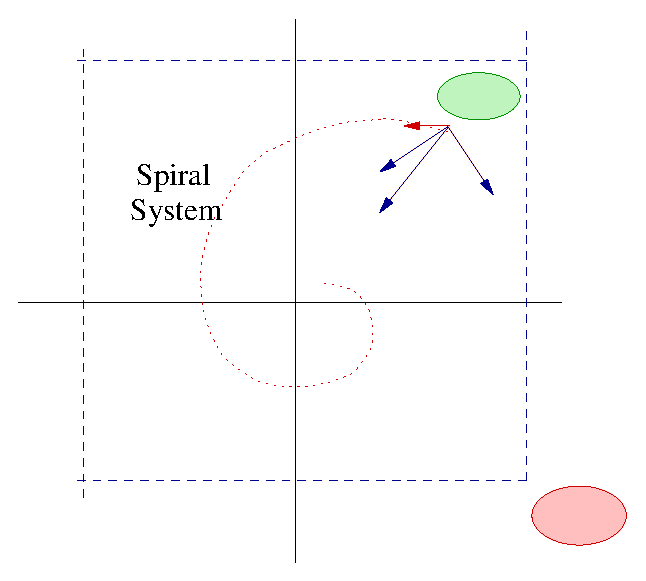
\includegraphics[angle=0,scale=0.3]{spiral}
\\
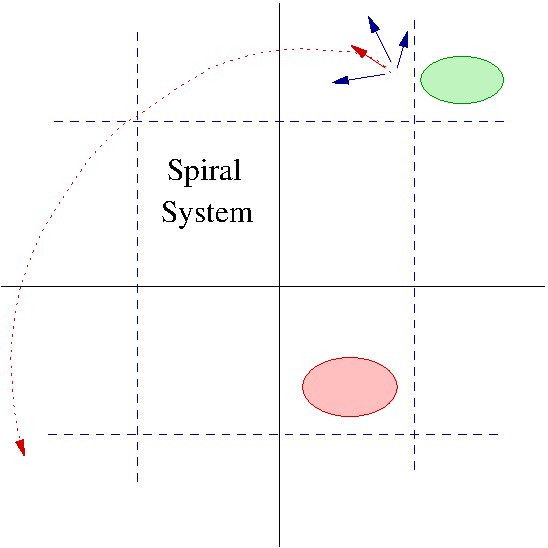
\includegraphics[angle=0,scale=0.3]{spiral-out}
\end{minipage}
&
\begin{minipage}{1.4in}
\small{
\begin{tabular}{|p{0.34in}|p{0.33in}|p{0.33in}|}
\hline
Class & $\frac{d\vec{x}}{dt}$ & RelAbs
\\
\hline \hline
\parbox{0.34in}{Timed System} & 
\parbox{0.34in}{$\dot{x}=1$,\\$\dot{y} = 1$} & 
\parbox{0.45in}{$x'-x=\\y'-y$}
\\
\hline
\parbox{0.34in}{Multirate System} & 
\parbox{0.34in}{$\dot{x}=2$,\\$\dot{y}=3$} & 
\parbox{0.33in}{$\frac{x'-x}{2} = \\ \frac{y'-y}{3}$}
\\
\hline
\parbox{0.34in}{Linear Hybrid System} & 
\parbox{0.36in}{$\dot{\vec{x}} = A\vec{x}$} & 
\parbox{0.33in}{$(0 \leq p'\leq p$}
\\
\hline
$\ldots$ & $\ldots$ & $\ldots$
\\
\hline
\end{tabular}

\bigskip

On Hybrid System benchmarks, verification time reduces from
~{\cem{10 hours}} to a {\cem{few minutes}} ({\crm{100x}} improvement).
}
\end{minipage}
\end{tabular}

\end{slide}
% -------------------------------------------------------
\begin{slide}
\heading{Demo: TGC Example}

Consider a {\crm{train-gate-controller}} system: Is it {\cem{safe}}?
\hfill{\small{From [Dutertre and Sorea, 2004]}}

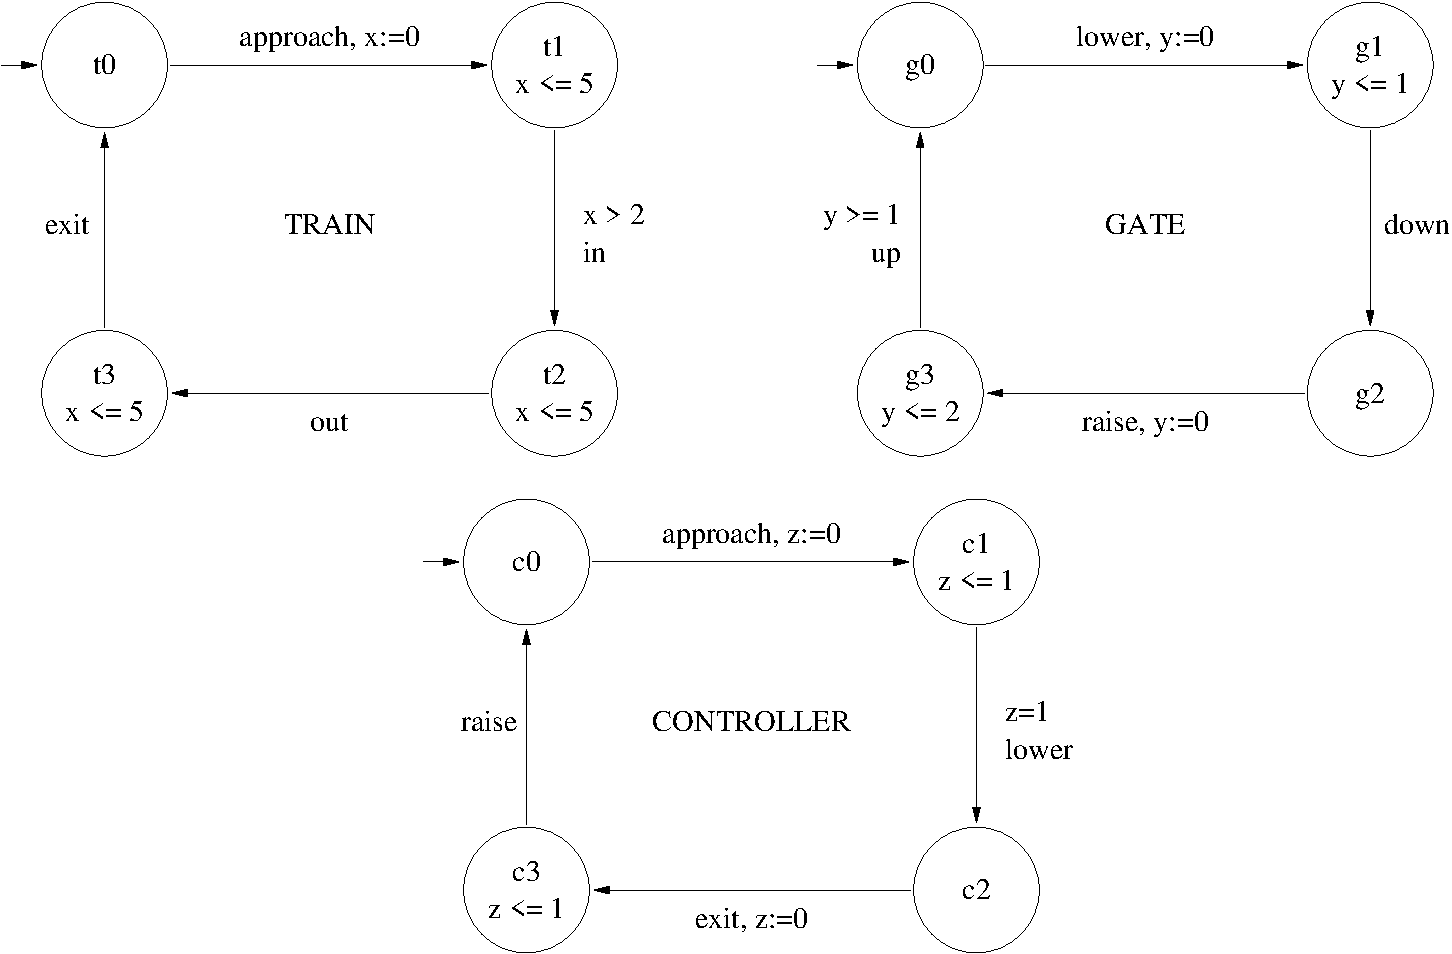
\includegraphics[angle=0,scale=0.38]{tgc}
\end{slide}
% -------------------------------------------------------
\begin{slide}
\heading{Demo: Navigation Example}

\begin{tabular}{cc}
\begin{minipage}{2.7in}
Consider a {\crm{robot}} moving in a 2d space.

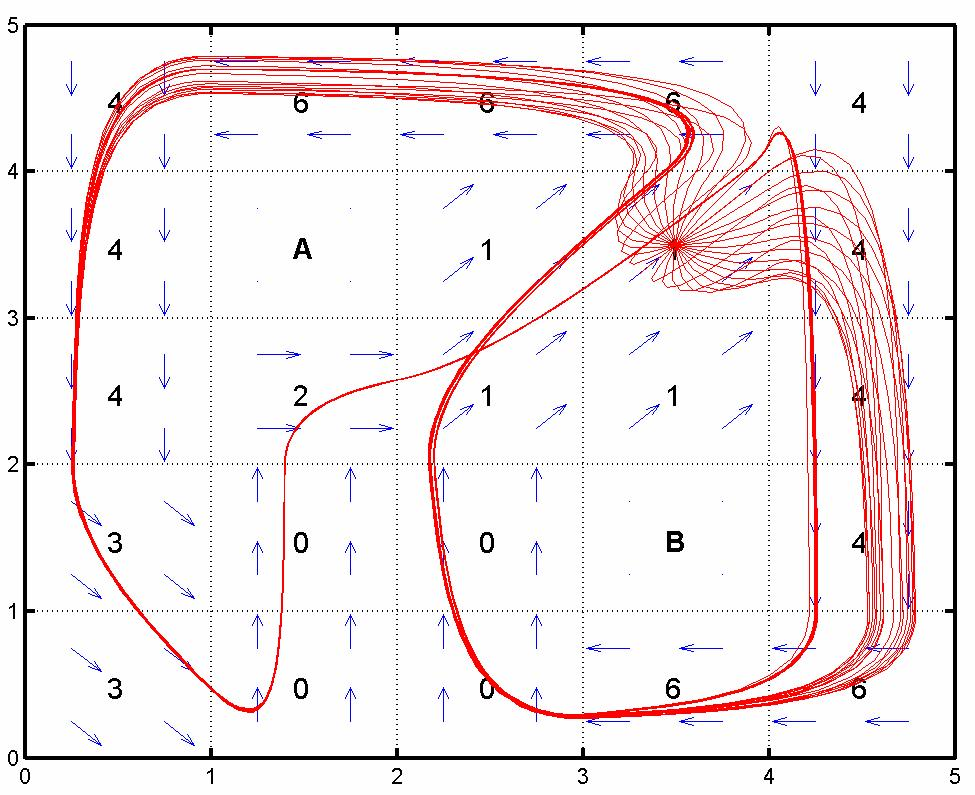
\includegraphics[angle=0,scale=0.2]{nav.jpeg}
\end{minipage}
&
\begin{minipage}{1.7in}
It should reach {\crm{A}}, while avoiding {\cem{B}}.

Dynamics:
\begin{eqnarray*}
\dot{\vec{x}} & = & \vec{v}
\\
\dot{\vec{v}} & = & A (\vec{v} - \vec{v}_d)
\end{eqnarray*}
The direction $\vec{v}_d$ depends on the position in the grid

Can verify instances in minutes using HSAL RelAbs and sal-inf-bmc

\hfill{\small{From [Ansgar and Ivancic, 2004]}}
\end{minipage}
\end{tabular}

\end{slide}
% -------------------------------------------------------
\begin{slide}
\heading{Backup: Abstraction vs RelAbstraction}

\begin{tabular}{cc}
\begin{minipage}[c]{0.6\linewidth}
\begin{center}
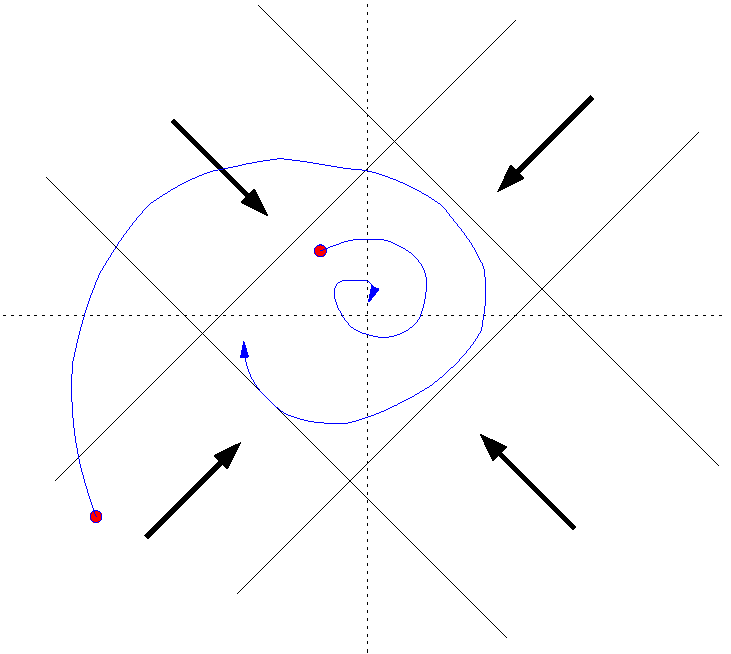
\includegraphics[angle=0,scale=0.5]{relabs-old}
\end{center}
\end{minipage}
&
\begin{minipage}[c]{0.35\linewidth}
Two methods for abstracting continuous/hybrid systems
\begin{itemize}
\item
 {\cem{predicate abstraction}}:  Implemented in HybridSAL
\item
 {\cem{relational abstraction}}: New approach that we will demonstrate here
\end{itemize}
\end{minipage}
\end{tabular}

\end{slide}
% -------------------------------------------------------
\begin{slide}
\heading{Abstraction for Open Systems}
\subheading{Relational Abstraction}

Abstract model defines how the {\cem{input}}
{\crm{relates}} to the {\cem{output}}

\begin{eqnarray}
 \frac{d\vec{x}}{dt} & = & f(\vec{x})
\\ & \Downarrow &
\\ 
 \vec{x}\;\rightarrow\;\vec{y} & \mbox{ if } &
 \vec{x},\vec{y} \mbox{ are related by } R(\vec{x},\vec{y})
\end{eqnarray}

\bigskip
Example:
\begin{eqnarray}
 \frac{dx}{dt} & = & -x
\\ & \Downarrow &
\\ 
 \vec{x}\;\rightarrow\;\vec{y} & \mbox{ if } &
(x \leq y < 0) \vee (0 < y \leq x) 
\end{eqnarray}

\end{slide}
% -------------------------------------------------------
\begin{slide}
\heading{Computing Relational Abstractions}

Suppose dynamics are $\frac{d\vec{x}}{dt} = A\vec{x}$

\begin{itemize}
\item Compute left eigenvector $\vec{c}^T$ of $A$
$$  \vec{c}^T A  = \lambda \vec{c}^T $$
\item
 Note that 
$$
 \frac{d(\vec{c}^T \vec{x})}{dt} =
 \vec{c}^T\frac{d\vec{x}}{dt} =
 \vec{c}^T A\vec{x} = \lambda \vec{c}^T\vec{x}
$$
\item
 Thus, we can relate the initial value of $c^T\vec{x}$ 
 and its future value $c^T\vec{x}'$ as follows:
$$
 0 < \vec{c}^T\vec{x}' \leq \vec{c}^T\vec{x}  \;\vee\;
 0 > \vec{c}^T\vec{x}' \geq \vec{c}^T\vec{x} 
$$
if $\lambda < 0$.  And if $\lambda > 0$, then $\vec{x},\vec{x}'$ swap places.
\end{itemize}

This idea generalizes to $\frac{d\vec{x}}{dt} = A\vec{x} + \vec{b}$

\end{slide}
% -------------------------------------------------------
\begin{slide}
\heading{Computing Relational Abstractions 2}

Suppose dynamics are $\frac{d\vec{x}}{dt} = A\vec{x}$

Suppose we have generated relations for all real eigenvalues

Now suppose there is a complex eigenvalue $a + b\iota$

\begin{itemize}
\item Find two vectors $\vec{c}^T$ and $\vec{d}^T$ such that
\begin{eqnarray*}
 \left(\begin{array}{c}
 \frac{d\vec{c}^T\vec{x}}{dt} \\
 \frac{d\vec{d}^T\vec{x}}{dt} 
 \end{array}\right)
 & = & 
  \left(\begin{array}{cc}
   a & -b \\ b & a
  \end{array}\right)
 \left(\begin{array}{c}
 \frac{d\vec{c}^T\vec{x}}{dt} \\
 \frac{d\vec{d}^T\vec{x}}{dt} 
 \end{array}\right)
\end{eqnarray*}

\item
 Thus,
 the values of $\vec{c}^T\vec{x}$ and $\vec{d}^T\vec{x}$ 
 spiral in (or spiral out) if $a < 0$ (respectively if $a > 0$) 

\item
 Hence, we can relate their initial values to their future values
$$
 (\vec{c}^T \vec{x})^2 + 
 (\vec{d}^T \vec{x})^2 
 \geq
 ({\vec{c}}^{T} \vec{x}')^2 + 
 ({\vec{d}}^{T} \vec{x}')^2 
$$
if $a < 0$, and the inequalities are reversed if $a > 0$
 
\end{itemize}

\end{slide}
% -------------------------------------------------------
\begin{slide}
\heading{Qualitative vs Relational Abstraction}

Consider $\dot{x} = -x$

Qualitative abstraction:
\\
if $qx = pos$ then $qx' \in \{pos,zero\}$
\\
if $qx = neg$ then $qx' \in \{neg,zero\}$
\\
if $qx = zero$ then $qx' = zero$

\bigskip
Relational abstraction:
\\
$0 \leq x' \leq x \;\vee\; 0 \geq x' \geq x$

\bigskip
If initially $x = 5$, then qualitative abstraction
can prove $x$ is never $neg$

\bigskip
If initially $x = 5$, then relational abstraction
can prove $x$ remains between $0$ and $5$
\end{slide}
% -------------------------------------------------------
\begin{slide}
\heading{Preliminary Demo of Timed Relational Abstraction}

{\cem{New}}: First version of {\cem{Timed Relational Abstraction}}

\medskip
{\cem{Why TRA?}} 
Would a controller that is designed and verified to be stable
in the {\cem{continuous domain}}, but implemented on a
{\cem{time triggered}} architecture, still maintain stability?

\medskip
{\cem{What is TRA?}} 
Abstraction of $dx(t)/dt = f(x)$ by a {\cem{relation}}
$R(x(0),x(T))$ that relates all possible pairs
$x(0),x(T)$, where $T$ is the {\cem{sampling period}}

\end{slide}
% -------------------------------------------------------
\begin{slide}
\heading{Example 1: Timed Proportional Controller}

Consider plant $\frac{dx}{dt} = 5*x + u$

Consider a P-controller $u = -30*x$

This is clearly stabilizing in the continuous domain.

Time-triggered implementation of this controller need
not be provably stabilizing.

When $T = 0.01$, the controller is still stabilizing

When $T = 0.1$, it is not so

\end{slide}
% -------------------------------------------------------
\begin{slide}
\heading{Example 2: Timed PI Controller}

Consider plant $\frac{dx}{dt} = 5*x + u$

Consider a PI-controller $u = -30*x - y$,
where $\frac{dy}{dt} = x$

When $T = 0.05$, the controller is stabilizing

When $T = 0.1$, the controller is stabilizing

When $T = 0.5$, it is not so

\end{slide}
% -------------------------------------------------------
\begin{slide}
\heading{Example 3: Inverted Pendulum}

\end{slide}
% -------------------------------------------------------
\end{document}
